\section{Completed million-event validation}
\label{sec:results}

\subsection{Processes, common inputs and analysis definitions}
The numerical study uses proton collisions at $13\,\mathrm{TeV}$ and
five processes at NLO in QCD:
\begin{align*}
 pp&\to ZZ, & pp&\to e^+e^-, & pp&\to t\bar t,\\
 pp&\to tj\quad(\text{t channel}), & pp&\to W^+b\bar b.
\end{align*}
The first four use the five-flavour model
\code{\detokenize{loop_sm-no_b_mass}} and
\code{\detokenize{MSTW2008nlo90cl/0}} (LHAPDF ID 21150).
Wbb uses \code{\detokenize{loop_sm}} with $m_b=4.7\GeV$ and
\code{\detokenize{MSTW2008nlo68cl_nf4/0}} (ID 23300).
The PDF definitions are those of Refs.~\cite{MSTW,LHAPDF}; the central
member and its exact files, not the confidence-level label alone,
determine each calculation. The actual measured shower-coupling flavour
convention is specified in the mass section: the four-flavour hard/PDF
calculation is not a claim of a fully nf4 running-coupling shower.

The single-top command is exactly
\begin{lstlisting}
p p > t j $$ w+ w- [QCD]
\end{lstlisting}
with $p$ and $j$ including $b,\bar b$ in the 5FS. It contains top
production, not the charge-conjugate antitop sample. All its generation
cuts, including hidden PDG cuts, are disabled. The Wbb command is
\begin{lstlisting}
p p > w+ b b~ QCD=2 QED=1 [QCD]
\end{lstlisting}
The DY run has $m_{e^+e^-}>60\GeV$. Other physical generation cuts are
disabled for these samples. Tops and electroweak bosons are stable.
Renormalization and factorization scales are $H_T/2$, with the generator's
transverse-mass sum prescription, and scale/PDF reweighting is off.
The requested integration accuracy is $0.001$, the event-job target is
10,000, and all folding factors are one. These numerical targets are not
an estimate of the matching uncertainty.

Each process has an ordinary and a Delta source of exactly $10^6$
events: ten million source event records in total. Repeated hard identities
are allowed and are paired with an explicit queue. For every cohort,
the postprocessor uses the corresponding unchanged source and freezes
one decision for every proposal. Accepted events are shuffled into a
single LHE file and retain their original signed cross-section weights.
There is no top-up to one million accepted events and no rescaling to the
number of survivors.

Jets are anti-$k_t$ with $R=0.4$, using FastJet core
and the analysis definitions described below~\cite{AntiKt,FastJet}.
No hadronisation, particle decays, MPI, primordial transverse momentum,
colour reconnection, QED/weak showers or resonance radiation is enabled.
Beam remnants are constructed in the full-shower analysis for global
momentum closure. No HepMC or full-shower event file is written: every
event is analyzed in memory and only histograms, moments and diagnostics
are saved.

For ZZ, the Z bosons are ordered in transverse momentum. DY uses the
electron and positron; top pairs use the top and antitop. Radiation jets
include final quarks of absolute PDG code at most five and gluons,
excluding the stable tops. Wbb uses the stable W, b and bbar as three
objects. Its pair masses, recoil and angular variables use $b\bar b$;
the full-system quantities use $W^+b\bar b$. Its radiation jets remove
bottom partons before clustering, while separate inclusive jet plots
include them. The former are parton-level radiation diagnostics, not a
definition of an experimental b-tagged jet observable.

In single top, the leading inclusive light-parton jet is an
infrared-safe spectator \emph{proxy}, not an ancestry tag. It can be a
radiation jet after showering. The hard system is $t+j_1$ and the
additional-radiation plots show the second jet, with zero transverse
momentum if absent. A leading jet already exists at Born level, so using
it as an extra-radiation variable would obscure the matching test.
Radiation-jet and inclusive all-jet rapidities require $\pt>20\GeV$;
hard-object rapidities, including the leading single-top jet proxy, have
no such cut. The momentum spectra retain
the zero/no-jet entries. Soft plots use uniform $0.5\GeV$ bins from zero
to $50\GeV$, except for top pairs, whose corresponding range is
$0$--$150\GeV$ with uniform $1\GeV$ bins. Broad spectra and every
underflow/overflow/missing counter are retained.

\subsection{Rates and the removal/veto balance}
\label{sec:rates}
Table~\ref{tab:rates} gives the signed sample sums. The changes arise at
the removal/veto stage: a complete shower does not alter the frozen
selection or its event weights. The first and full sample sums agree to
numerical precision because each relevant event is consumed exactly
once. This is a check of event handling and normalization; it is not a
proof that the two matching prescriptions have equal rates.
\begin{table}[tbp]
\centering\small
\begin{tabular}{llrrrr}
\toprule
Process & Source & Retained & $\sigma_{\rm MC}$ [pb] & $\sigma_{\rm MAc}$ [pb] & Change [\%]\\
\midrule
$ZZ$ & ordinary & 975,657 & 14.2002 & 14.2883 & +0.621\\
$ZZ$ & $\Delta$ & 989,589 & 14.1735 & 14.1959 & +0.158\\
DY & ordinary & 961,679 & 1859.2 & 1876.09 & +0.908\\
DY & $\Delta$ & 983,990 & 1862.08 & 1863.92 & +0.099\\
$t\bar t$ & ordinary & 726,454 & 678.195 & 723.098 & +6.621\\
$t\bar t$ & $\Delta$ & 954,264 & 675.244 & 673.504 & -0.258\\
$tj$ & ordinary & 571,819 & 132.387 & 154.68 & +16.839\\
$tj$ & $\Delta$ & 697,436 & 132.49 & 145.698 & +9.970\\
$W^+b\bar b$ & ordinary & 828,798 & 487.904 & 480.943 & -1.427\\
$W^+b\bar b$ & $\Delta$ & 896,189 & 484.774 & 478.306 & -1.334\\
\bottomrule
\end{tabular}
\caption{Completed million-event common-source samples. Every source has $10^6$ events; retained events keep their original signed weights. Cross sections are the sums of the event weights, rather than a renormalization to the accepted count. The first-emission and full-shower sums agree to numerical precision.}
\label{tab:rates}
\end{table}

\begin{table}[tbp]
\centering\small
\begin{tabular}{llrrr}
\toprule
Process & Source & H removal [pb] & S veto [pb] & Combined [pb]\\
\midrule
$ZZ$ & ordinary & +0.22676 & -0.13862 & +0.088134\\
$ZZ$ & $\Delta$ & +0.086398 & -0.063997 & +0.022402\\
DY & ordinary & +46.659 & -29.773 & +16.886\\
DY & $\Delta$ & +16.335 & -14.491 & +1.8442\\
$t\bar t$ & ordinary & +165.81 & -120.91 & +44.903\\
$t\bar t$ & $\Delta$ & +16.526 & -18.265 & -1.7394\\
$tj$ & ordinary & +73.879 & -51.587 & +22.292\\
$tj$ & $\Delta$ & +41.882 & -28.673 & +13.209\\
$W^+b\bar b$ & ordinary & +46.84 & -53.802 & -6.9619\\
$W^+b\bar b$ & $\Delta$ & +25.217 & -31.685 & -6.4679\\
\bottomrule
\end{tabular}
\caption{Changes of the signed cross section from H removal alone, S rejection alone, and their combination. The first two columns add to the last; rejected negative S weights contribute with the opposite sign to rejected positive S weights. No events are rescaled.}
\label{tab:effects}
\end{table}


The effect columns in Table~\ref{tab:effects} make the compensation
directly measurable. For ordinary DY, H removal adds about $46.66\pb$
and S rejection removes about $29.77\pb$, leaving $+16.89\pb$.
Consequently, the compensation is not close to an exact cancellation in
that sample. The small $+0.908\%$ shift relative to the large inclusive
DY rate should not conceal the much larger mismatch relative to the
removed H contribution. With Delta, the corresponding shifts are
$+16.34\pb$ and $-14.49\pb$, leaving $+1.84\pb$.

Ordinary ZZ changes by $+0.621\%$, reduced to $+0.158\%$ in its Delta
cohort. Top pairs change by $+6.621\%$ without Delta and $-0.258\%$ with
Delta. The soft region extends over larger transverse momenta for this
massive coloured system, which motivates the wider uniform-binning
presentation. A fixed small colour-singlet plotting window would hide a
substantial part of that comparison.

Single top is the strongest finite-rate counterexample in this study:
$+16.839\%$ without Delta and $+9.970\%$ with Delta. H removal and S
veto plainly do not balance closely there. Wbb has the opposite net sign:
$-1.427\%$ without Delta and $-1.334\%$ with Delta. In both Wbb samples,
the signed S veto removes more than H removal adds. These results exclude
any universal assertion of exact cancellation or a universally
sub-percent finite effect for this implementation.

The ordinary and Delta source sums themselves are independently sampled
estimates from different source runs. Their difference is not an
event-by-event paired matching difference. The within-cohort percentages
in Table~\ref{tab:rates} are the relevant removal/veto comparison. The
tables do not quote generator integration errors as if they were the
uncertainty of these paired histogram sums, and they do not replace a
scale or matching-systematics study.

\subsection{The remaining negative weights}
\label{sec:remaining-negative}
\begin{table}[tbp]
\centering\small
\begin{tabular}{llrrrr}
\toprule
Process & Source & $N^-_{H,\rm source}$ & $N^-_{H,\rm retained}$ & $N^-_{S,\rm source}$ & $N^-_{S,\rm retained}$\\
\midrule
$ZZ$ & ordinary & 14,739 & 30 & 24,700 & 24,379\\
$ZZ$ & $\Delta$ & 5,748 & 13 & 23,843 & 23,629\\
DY & ordinary & 23,070 & 127 & 19,828 & 19,459\\
DY & $\Delta$ & 8,292 & 19 & 20,177 & 19,978\\
$t\bar t$ & ordinary & 151,332 & 52 & 39,290 & 33,313\\
$t\bar t$ & $\Delta$ & 20,807 & 0 & 54,109 & 53,143\\
$tj$ & ordinary & 243,601 & 4,981 & 42,602 & 31,131\\
$tj$ & $\Delta$ & 178,487 & 11,548 & 57,463 & 46,795\\
$W^+b\bar b$ & ordinary & 72,320 & 60 & 51,337 & 43,366\\
$W^+b\bar b$ & $\Delta$ & 41,996 & 275 & 56,981 & 52,147\\
\bottomrule
\end{tabular}
\caption{Global-sum campaign. Negative H and S event counts before and after the frozen decisions. These are counts, not integrals of negative densities. A zero in this finite sample does not prove that the residual vanishes throughout phase space.}
\label{tab:negatives}
\end{table}

Negative H events remain in every listed cohort except the finite
Delta top-pair sample. Their counts in Table~\ref{tab:negatives} follow
the bounded prescription, not an unconditional deletion of every
negative H. In particular, ordinary single top retains 4,981 negative H
events; Delta single top retains 11,548. Wbb retains 60 and 275,
respectively. The larger residual count with Delta in those two processes
is compatible with the algorithm: Delta changes the conditional source
law and the balance against the eligible leading kernel, not just an
overall number of negative H events.

For the same reason, the absence of negative H events in the sampled
Delta top-pair output is an empirical finite-sample statement. It does
not establish a pointwise positivity theorem for unsampled regions or
other processes. Comparing absolute residual counts alone is also not a
substitute for comparing their signed weight or their distribution over
phase space.

Negative S events remain in all ten samples. Some are rejected by the
same S decision that rejects positive events, but no step changes their
sign or constructs a generally positive Born coefficient. The surviving
sample is therefore not universally positive even when no negative H
event happens to remain. A smaller negative fraction can improve a
signed-weight statistical diagnostic; it is not sufficient evidence for
a better physical prediction if the cross section has also changed.

\subsection{How to read the first and full plots}
The first-step black curve is the complete unrejected proposal stream.
The H-only, S-only and combined masks share its events and kinematics.
They satisfy, in every bin and in each flow category,
\begin{equation}
  \Sigma_{\rm MAc}=\Sigma_{H\text{-only}}+
                   \Sigma_{S\text{-only}}-\Sigma_{\rm input}.
 \label{eq:plot-identity}
\end{equation}
This identity holds with the signed H residual included. It would be
wrong to make the H-only control by deleting all negative H events when
the actual combined algorithm retained some of them.

The full-shower black curve instead comes from the uninterrupted
original-source shower. Blue is the unrejected staged restart, orange
and green are the H-only and S-only selections of that same continued
population, and magenta is the accepted population. The full version of
Eq.~\eqref{eq:plot-identity} uses the blue population as input. A black
and blue difference is therefore not an H/S selection effect. It can
contain the first-profile mode-0 versus mode-2 difference, mass
presentation and scale import, loss of internal state at restart, and
the use of local recoil after the handoff.

Every ratio panel uses the corresponding combined MAcNLOPS curve as
denominator, including Delta+MAcNLOPS for the Delta cohort. Paired
covariance is included; a comparison of a curve with itself has unit
ratio and zero ratio variance where defined. Zero-denominator bins
remain undefined. Negative sums remain signed, and values whose
positive/negative cancellation is at roundoff level are not drawn as
spurious logarithmic tails. Unrestricted panels are accompanied by
ratio-zoom panels with off-scale triangles. Neither zooming nor flow
accounting changes the normalization of the plotted sample.

\subsection{What the observed differences do and do not diagnose}
Equation~\eqref{eq:finite-defect} identifies the relevant density mismatch
in the ordinary first-step construction, and its conditional extension
does so for Delta. It does not imply that the available histograms
separately measure every factor in $E_g/K_g$. The present campaign has
not reconstructed the exact multidimensional signed native emission
density or independently attributed a numerical percentage to each
potential mismatch.

In particular, the DY result cannot be explained merely by saying that
the source forgot the bogus Sudakov: both ordinary comparison branches
use the same source with that factor retained. Nor is it caused by a
normalization to the survivor count, since no such normalization is
performed. Plausible contributions to the mismatch include the NLO S
normalization and signs, genuine Sudakov suppression, starting-scale and
flavour mixtures, protected support, source G/spin structures, native PDF
and trial-acceptance policies, and the difference between the leading
analytic and actual accepted laws. The first/full controls then expose
additional presentation/profile/restart effects. A claim that exactly
one of these causes the observed DY or single-top shift would require
an additional targeted comparison that is not supplied by these plots.

The results are therefore informative even where agreement is poor:
they quantify the current prescription and show where its formal
leading argument is insufficient as a finite numerical guarantee. They
do not turn a $10$--$17\%$ effect into an established precision
prediction merely by calling it formally beyond NLO.

\subsection{Selected comparisons}
The following panels display the ordinary first-step spectrum and both
ordinary and Delta full spectra for every process. All the remaining
observables, unrestricted/zoom companions and standalone mechanism
panels are in the complete atlas. The 703 source figure files, including
the seven clearly separated historical panels, have individual hashes
in the portable source bundle.
\begin{figure}[p]
\centering
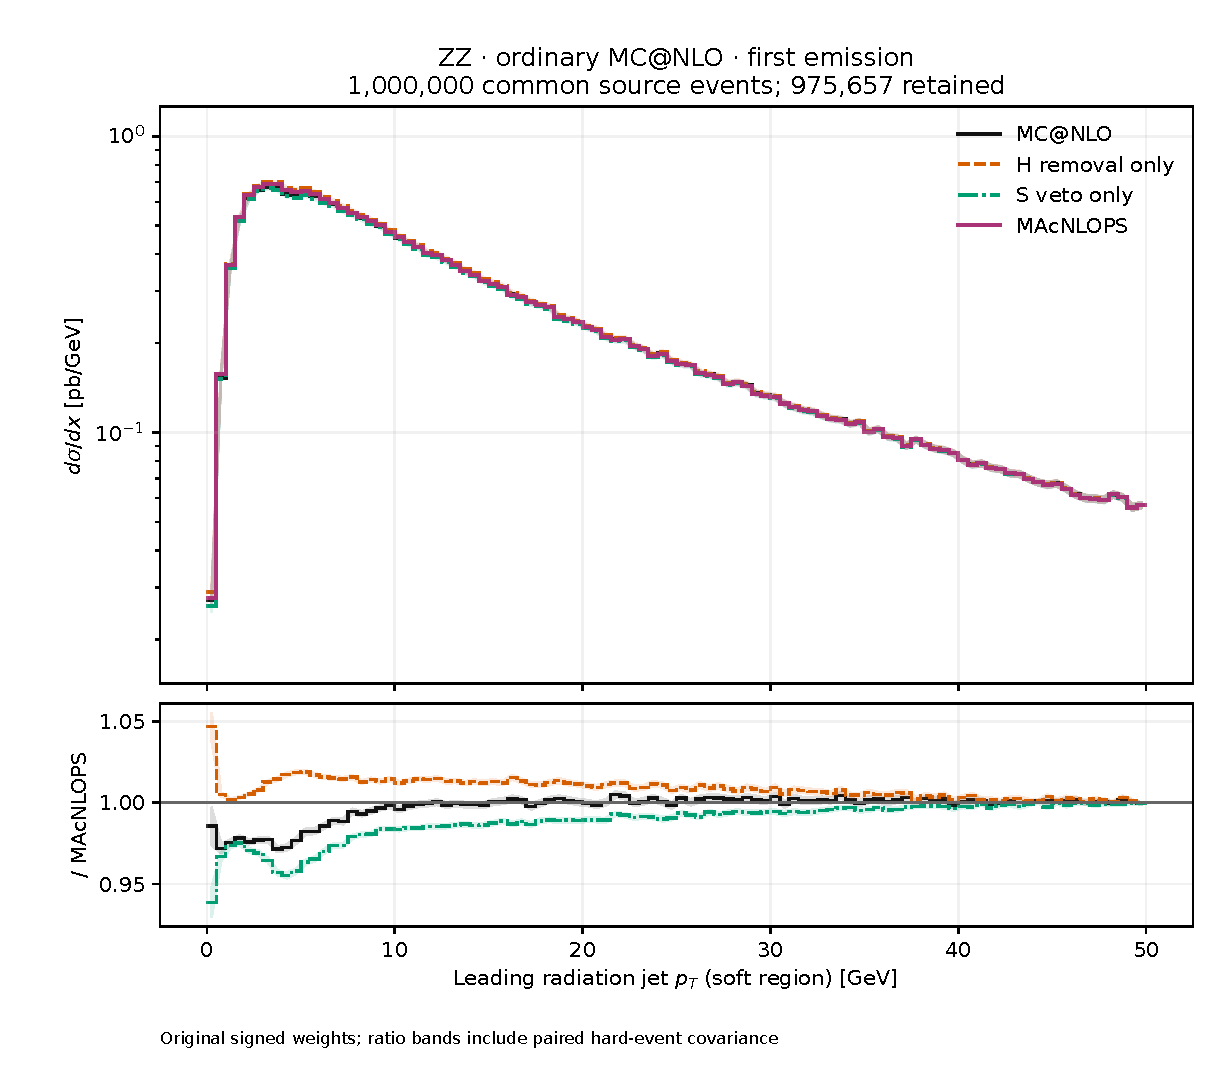
\includegraphics[width=.96\textwidth,height=.72\textheight,keepaspectratio]{figures/first/zz_ordinary/jet_pt_soft.pdf}
\caption{Global-sum campaign. ZZ (5FS), ordinary MC@NLO, first-emission proposal endpoint. The soft range is $0$--$50\GeV$ with uniform $0.5\GeV$ bins. The black curve is the complete unrejected first-step proposal control, not a separately initialized default-import shower. Orange and green isolate H removal and S veto. All ratios use the corresponding combined MAcNLOPS distribution as denominator. Original signed cross-section weights are preserved.}
\label{fig:zz-ordinary-first}
\end{figure}

\begin{figure}[p]
\centering
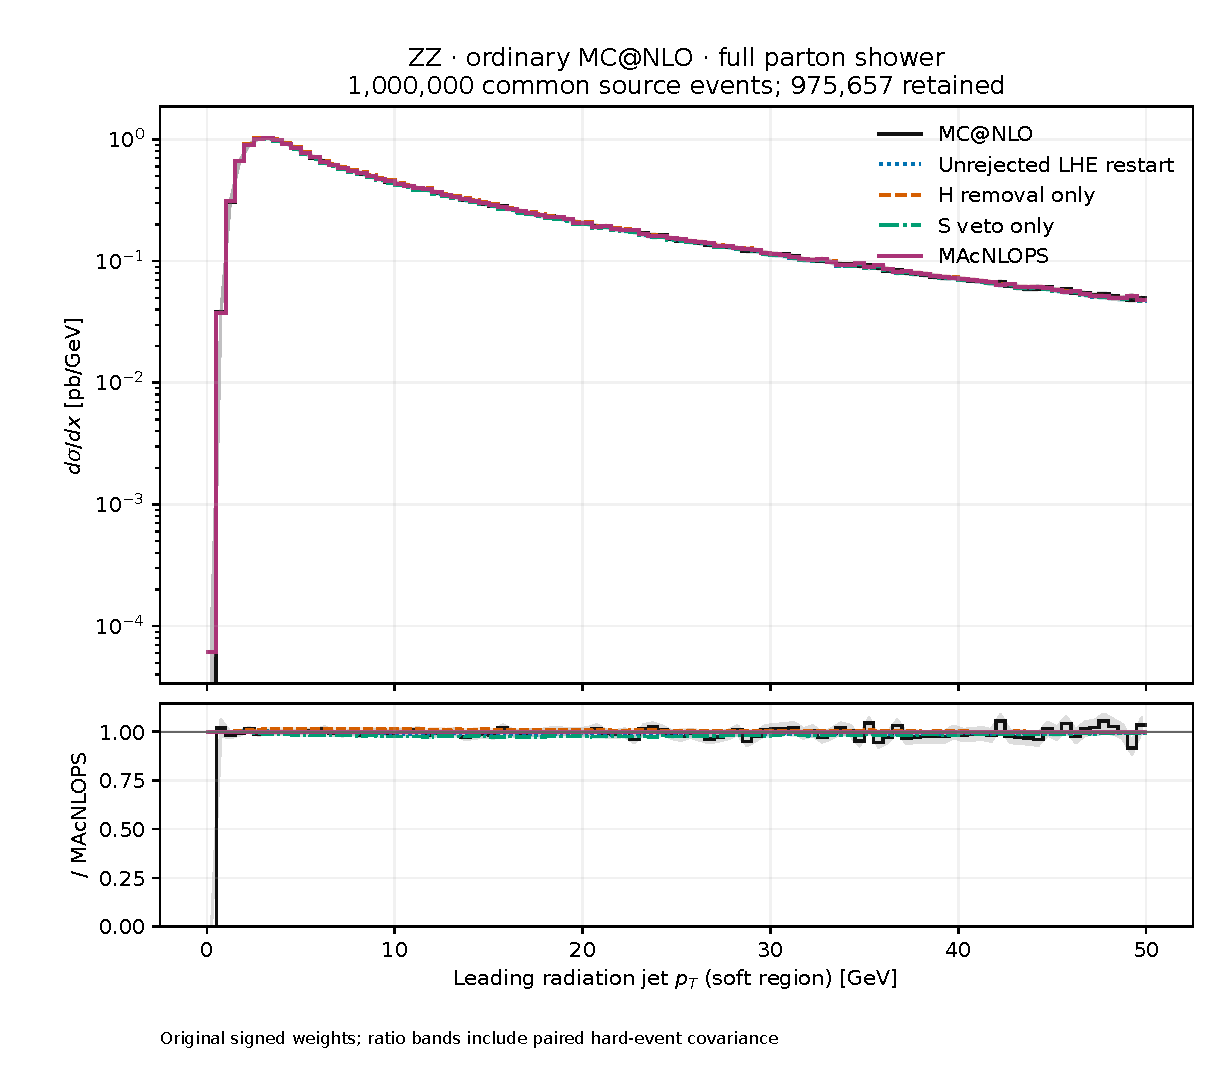
\includegraphics[width=.96\textwidth,height=.72\textheight,keepaspectratio]{figures/full/zz_ordinary/jet_pt_soft.pdf}
\caption{ZZ (5FS), ordinary MC@NLO, full parton shower. The soft range is $0$--$50\GeV$ with uniform $0.5\GeV$ bins. The black curve is the uninterrupted reference; blue is the unrejected staged restart. Orange and green isolate H removal and S veto. All ratios use the corresponding combined MAcNLOPS distribution as denominator. Original signed cross-section weights are preserved.}
\label{fig:zz-ordinary-full}
\end{figure}

\begin{figure}[p]
\centering
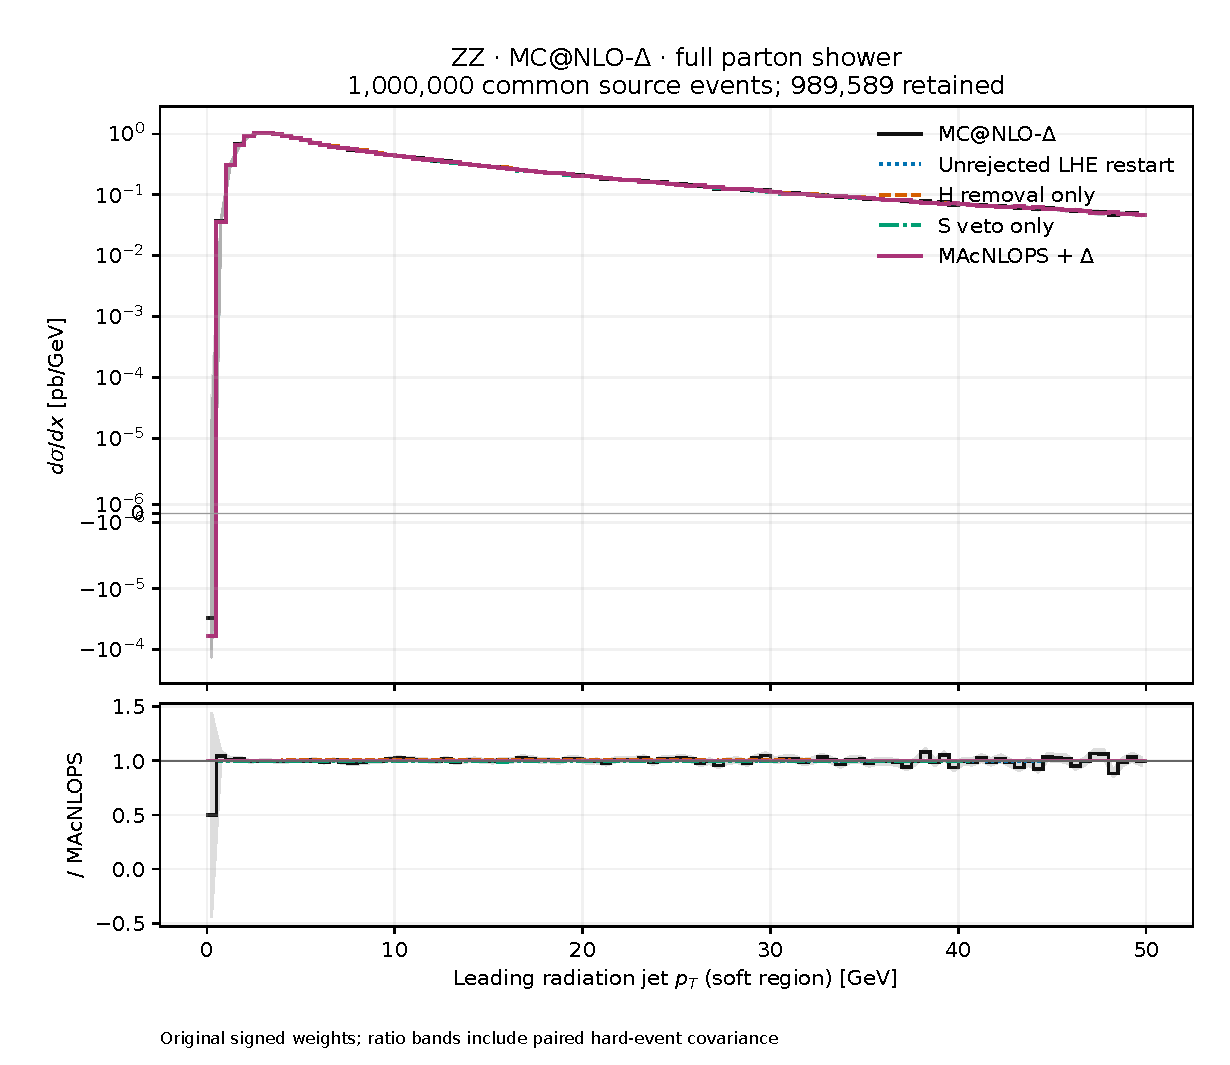
\includegraphics[width=.96\textwidth,height=.72\textheight,keepaspectratio]{figures/full/zz_delta/jet_pt_soft.pdf}
\caption{ZZ (5FS), MC@NLO-$\Delta$, full parton shower. The soft range is $0$--$50\GeV$ with uniform $0.5\GeV$ bins. The black curve is the uninterrupted reference; blue is the unrejected staged restart. Orange and green isolate H removal and S veto. All ratios use the corresponding combined MAcNLOPS distribution as denominator. Original signed cross-section weights are preserved.}
\label{fig:zz-delta-full}
\end{figure}

\begin{figure}[p]
\centering
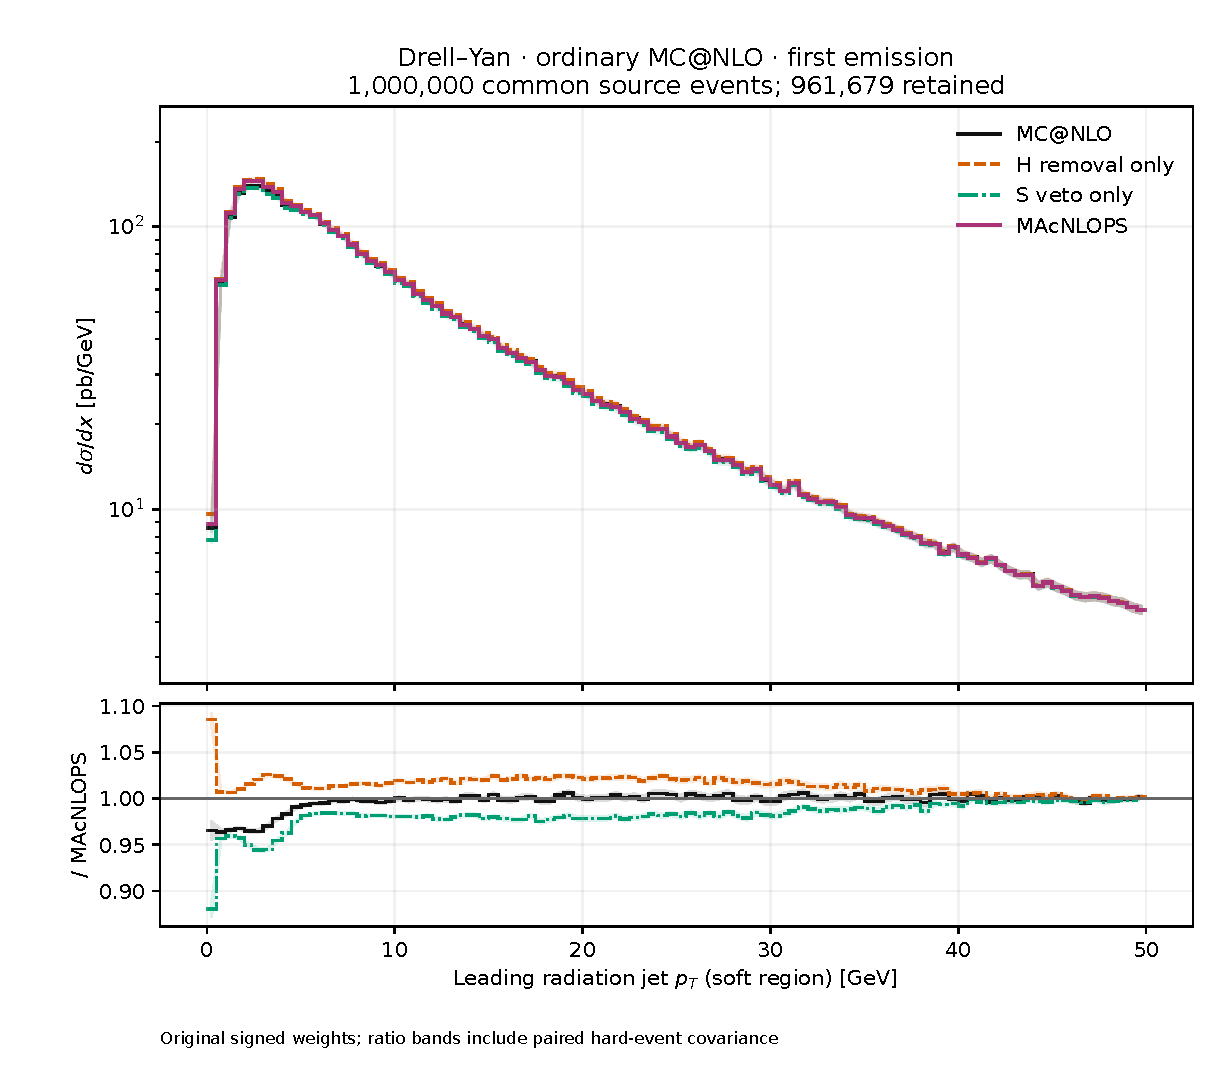
\includegraphics[width=.96\textwidth,height=.72\textheight,keepaspectratio]{figures/first/dy_ordinary/jet_pt_soft.pdf}
\caption{Drell-Yan (5FS), ordinary MC@NLO, first-emission proposal endpoint. The soft range is $0$--$50\GeV$ with uniform $0.5\GeV$ bins. The black curve is the complete unrejected first-step proposal control, not a separately initialized default-import shower. Orange and green isolate H removal and S veto. All ratios use the corresponding combined MAcNLOPS distribution as denominator. Original signed cross-section weights are preserved.}
\label{fig:dy-ordinary-first}
\end{figure}

\begin{figure}[p]
\centering
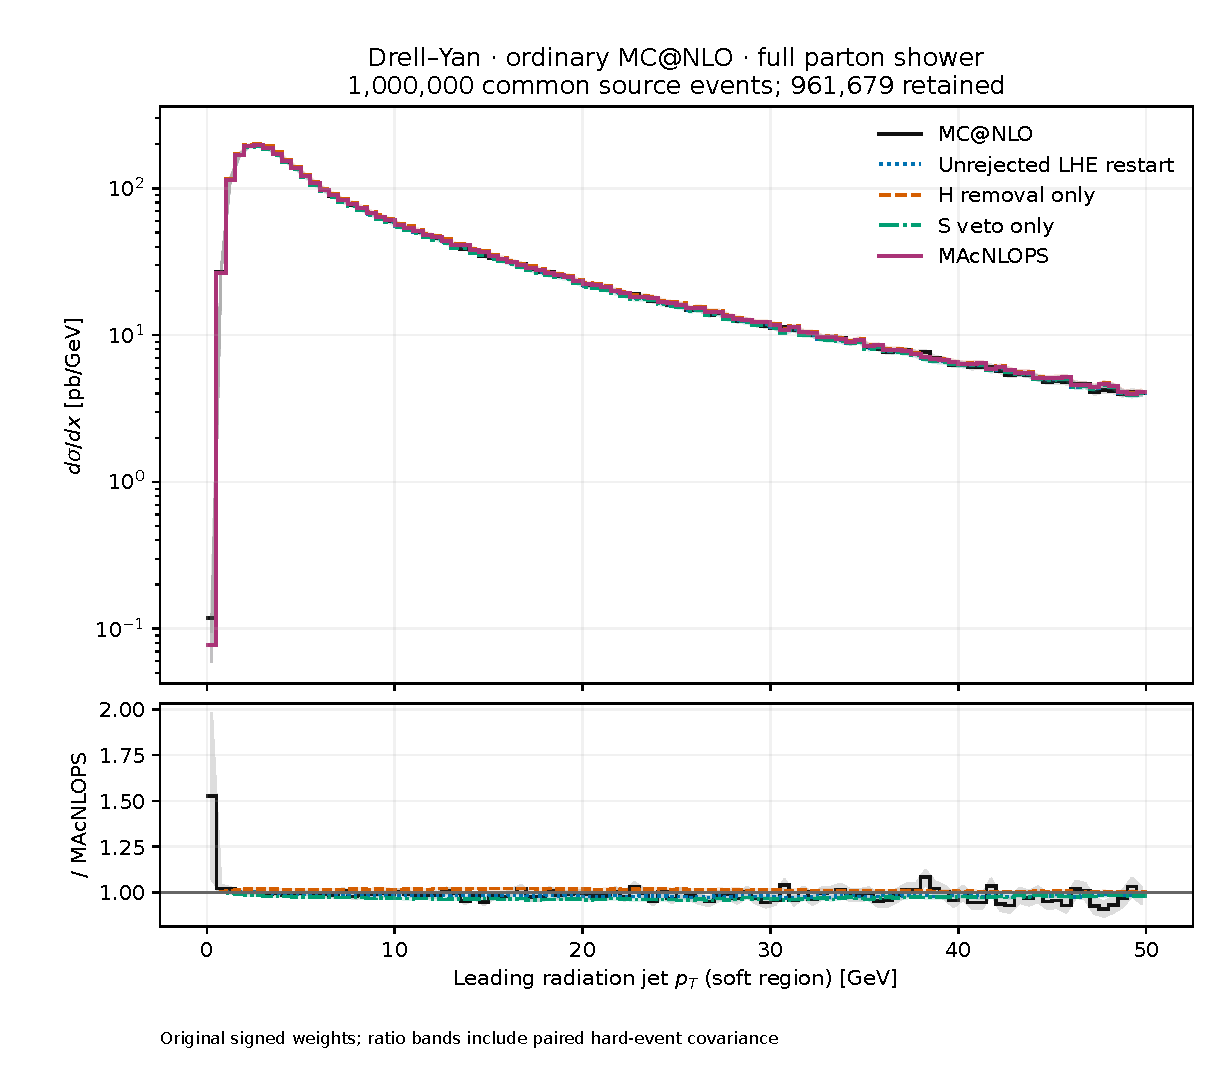
\includegraphics[width=.96\textwidth,height=.72\textheight,keepaspectratio]{figures/full/dy_ordinary/jet_pt_soft.pdf}
\caption{Global-sum campaign. Drell-Yan (5FS), ordinary MC@NLO, full parton shower. The soft range is $0$--$50\GeV$ with uniform $0.5\GeV$ bins. The black curve is the uninterrupted reference; blue is the unrejected staged restart. Orange and green isolate H removal and S veto. All ratios use the corresponding combined MAcNLOPS distribution as denominator. Original signed cross-section weights are preserved.}
\label{fig:dy-ordinary-full}
\end{figure}

\begin{figure}[p]
\centering
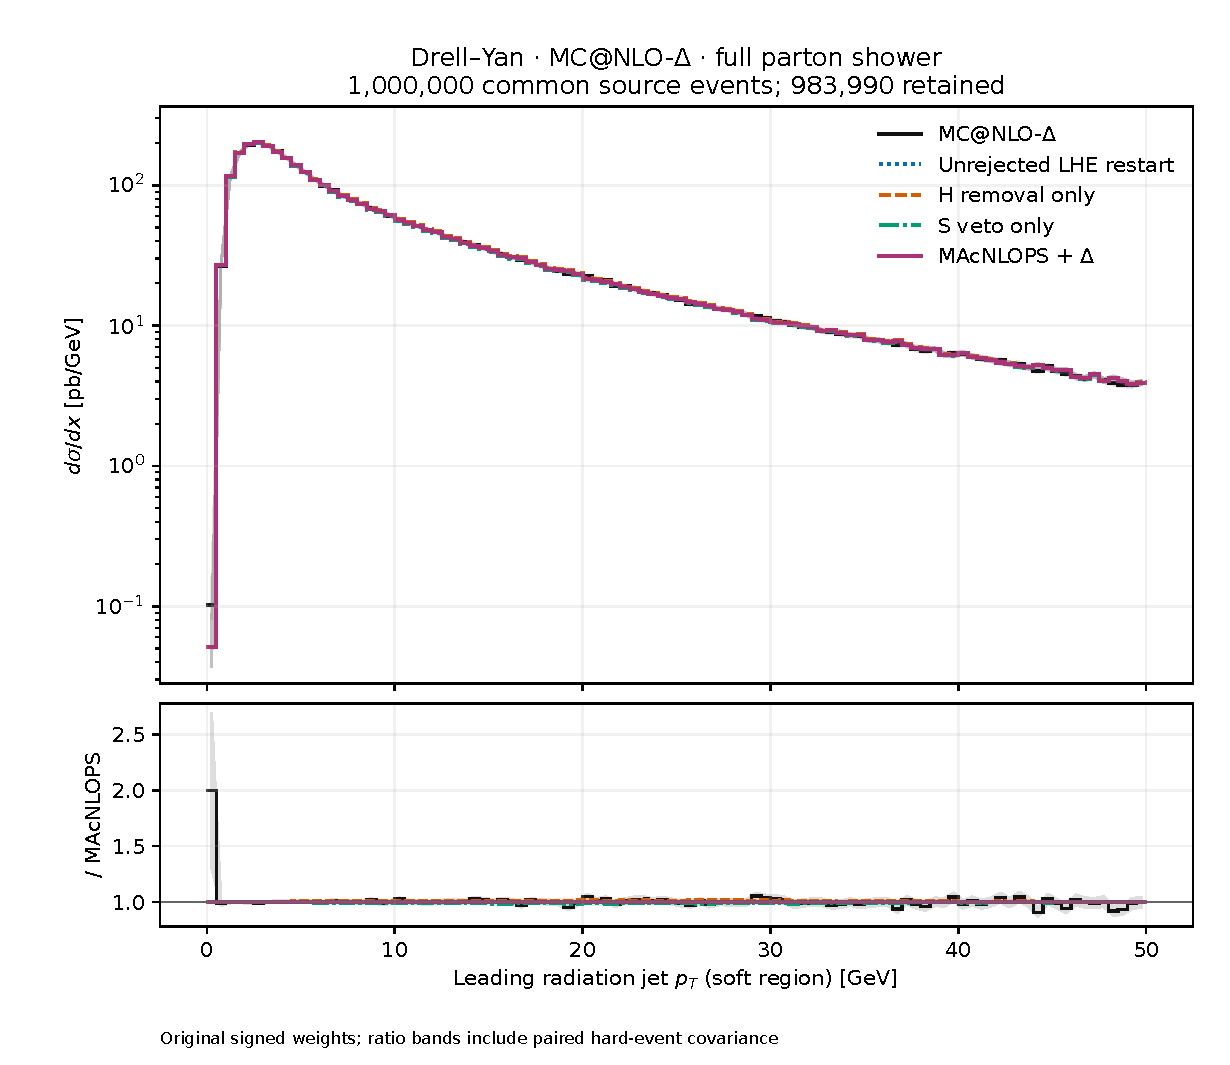
\includegraphics[width=.96\textwidth,height=.72\textheight,keepaspectratio]{figures/full/dy_delta/jet_pt_soft.pdf}
\caption{Drell-Yan (5FS), MC@NLO-$\Delta$, full parton shower. The soft range is $0$--$50\GeV$ with uniform $0.5\GeV$ bins. The black curve is the uninterrupted reference; blue is the unrejected staged restart. Orange and green isolate H removal and S veto. All ratios use the corresponding combined MAcNLOPS distribution as denominator. Original signed cross-section weights are preserved.}
\label{fig:dy-delta-full}
\end{figure}

\begin{figure}[p]
\centering
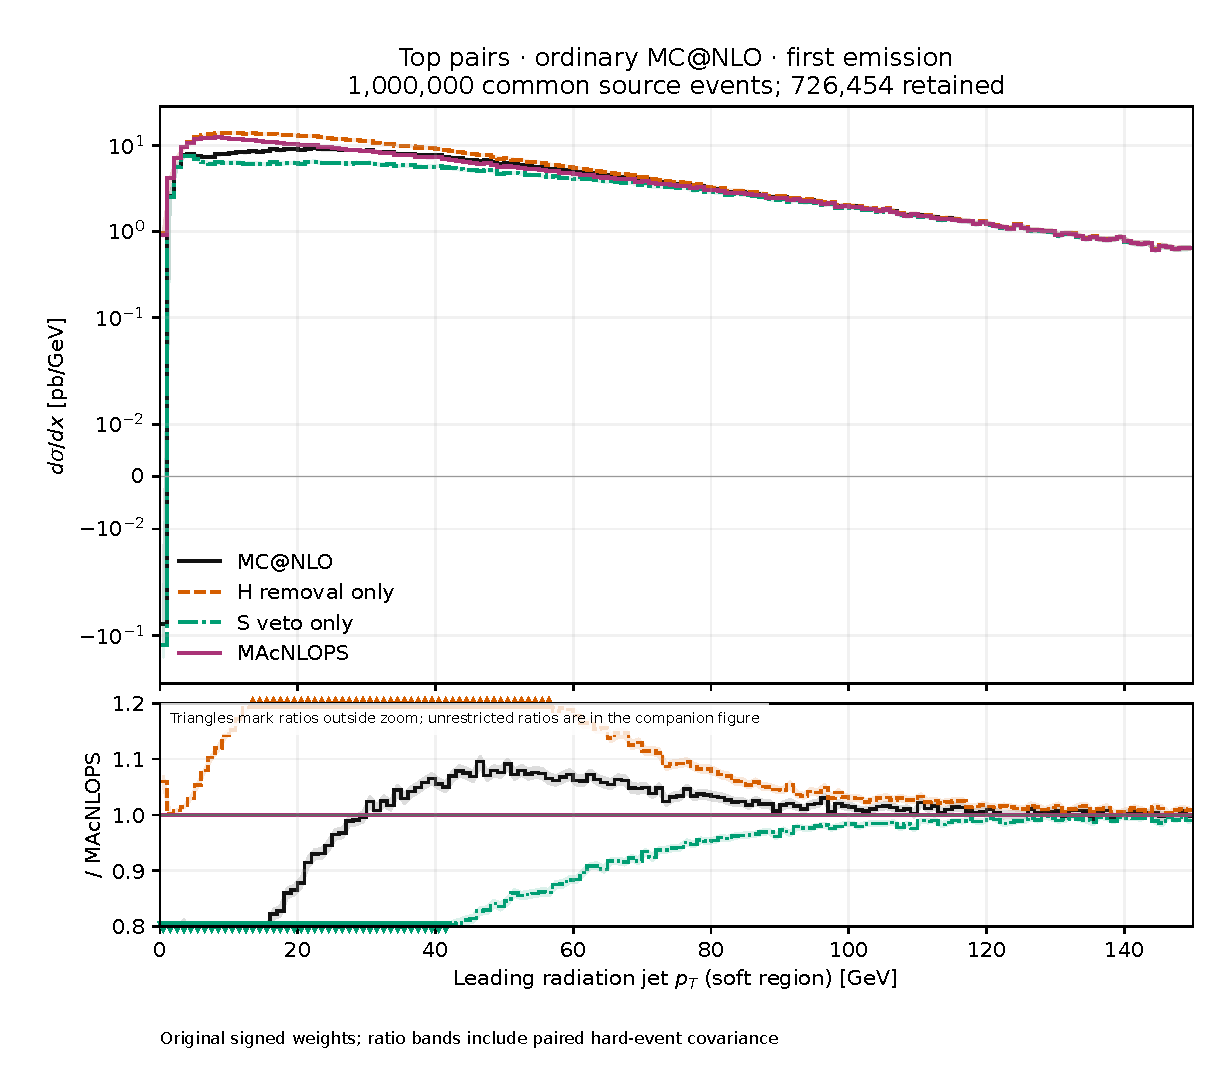
\includegraphics[width=.96\textwidth,height=.72\textheight,keepaspectratio]{figures/first/ttbar_ordinary/jet_pt_soft_ratio_zoom.pdf}
\caption{Global-sum campaign. Top pair (5FS), ordinary MC@NLO, first-emission proposal endpoint. The displayed soft range is $0$--$150\GeV$ with uniform $1\GeV$ bins. Triangles mark ratios outside the displayed zoom. The black curve is the complete unrejected first-step proposal control, not a separately initialized default-import shower. Orange and green isolate H removal and S veto. All ratios use the corresponding combined MAcNLOPS distribution as denominator. Original signed cross-section weights are preserved.}
\label{fig:ttbar-ordinary-first}
\end{figure}

\begin{figure}[p]
\centering
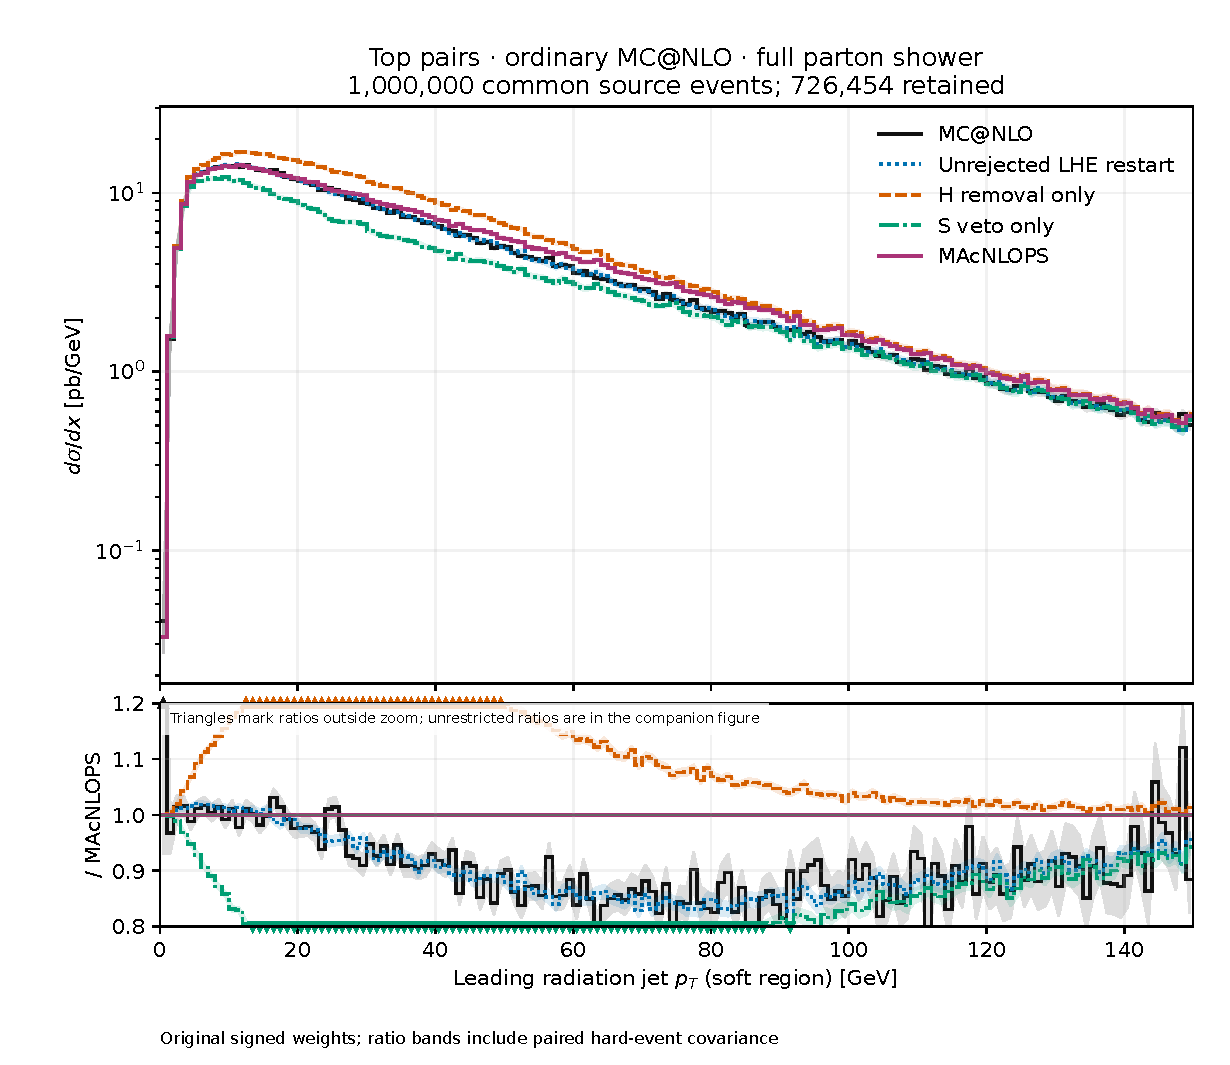
\includegraphics[width=.96\textwidth,height=.72\textheight,keepaspectratio]{figures/full/ttbar_ordinary/jet_pt_soft_ratio_zoom.pdf}
\caption{Top pair (5FS), ordinary MC@NLO, full parton shower. The displayed soft range is $0$--$150\GeV$ with uniform $1\GeV$ bins. Triangles mark ratios outside the displayed zoom. The black curve is the uninterrupted reference; blue is the unrejected staged restart. Orange and green isolate H removal and S veto. All ratios use the corresponding combined MAcNLOPS distribution as denominator. Original signed cross-section weights are preserved.}
\label{fig:ttbar-ordinary-full}
\end{figure}

\begin{figure}[p]
\centering
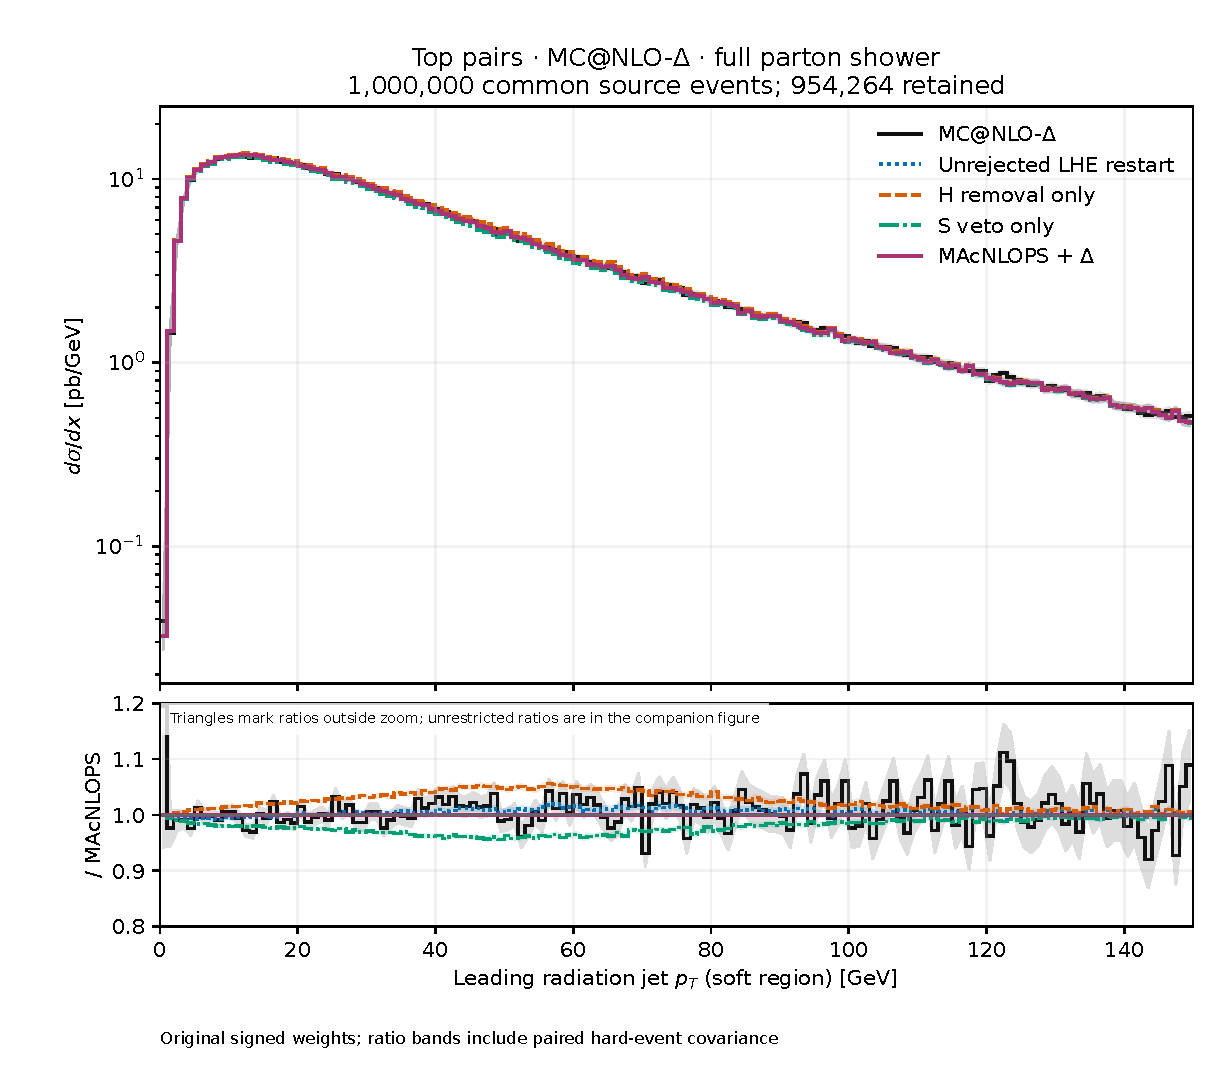
\includegraphics[width=.96\textwidth,height=.72\textheight,keepaspectratio]{figures/full/ttbar_delta/jet_pt_soft_ratio_zoom.pdf}
\caption{Global-sum campaign. Top pair (5FS), MC@NLO-$\Delta$, full parton shower. The displayed soft range is $0$--$150\GeV$ with uniform $1\GeV$ bins. Triangles mark ratios outside the displayed zoom. The black curve is the uninterrupted reference; blue is the unrejected staged restart. Orange and green isolate H removal and S veto. All ratios use the corresponding combined MAcNLOPS distribution as denominator. Original signed cross-section weights are preserved.}
\label{fig:ttbar-delta-full}
\end{figure}

\begin{figure}[p]
\centering
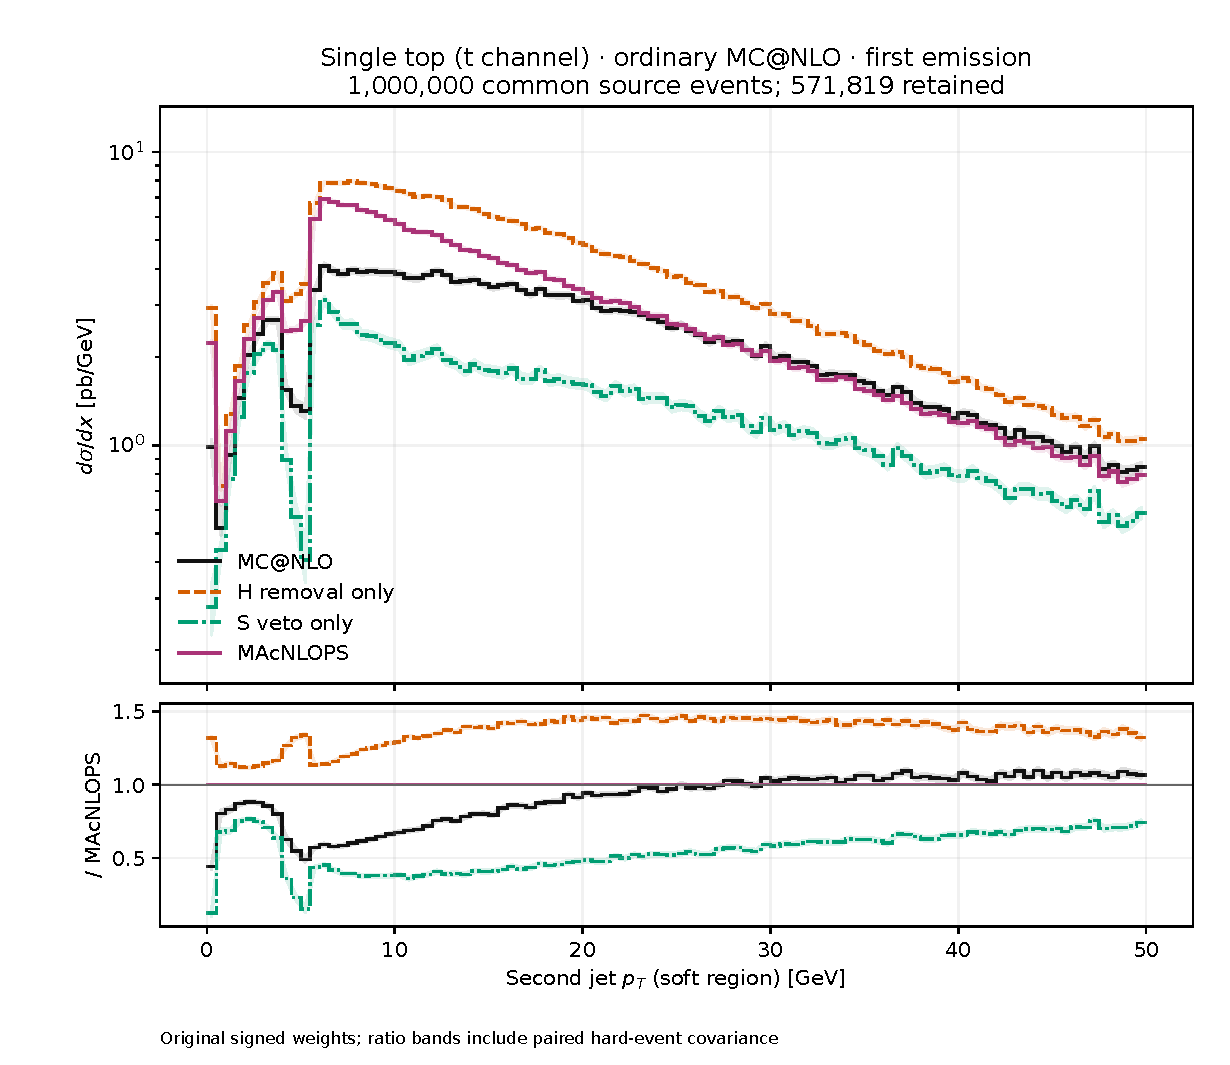
\includegraphics[width=.96\textwidth,height=.72\textheight,keepaspectratio]{figures/first/single_top_ordinary/jet_pt_soft.pdf}
\caption{Single top (5FS), ordinary MC@NLO, first-emission proposal endpoint. The second inclusive jet is shown; the leading jet is the spectator proxy. The soft range is $0$--$50\GeV$ with uniform $0.5\GeV$ bins. The black curve is the complete unrejected first-step proposal control, not a separately initialized default-import shower. Orange and green isolate H removal and S veto. All ratios use the corresponding combined MAcNLOPS distribution as denominator. Original signed cross-section weights are preserved.}
\label{fig:single_top-ordinary-first}
\end{figure}

\begin{figure}[p]
\centering
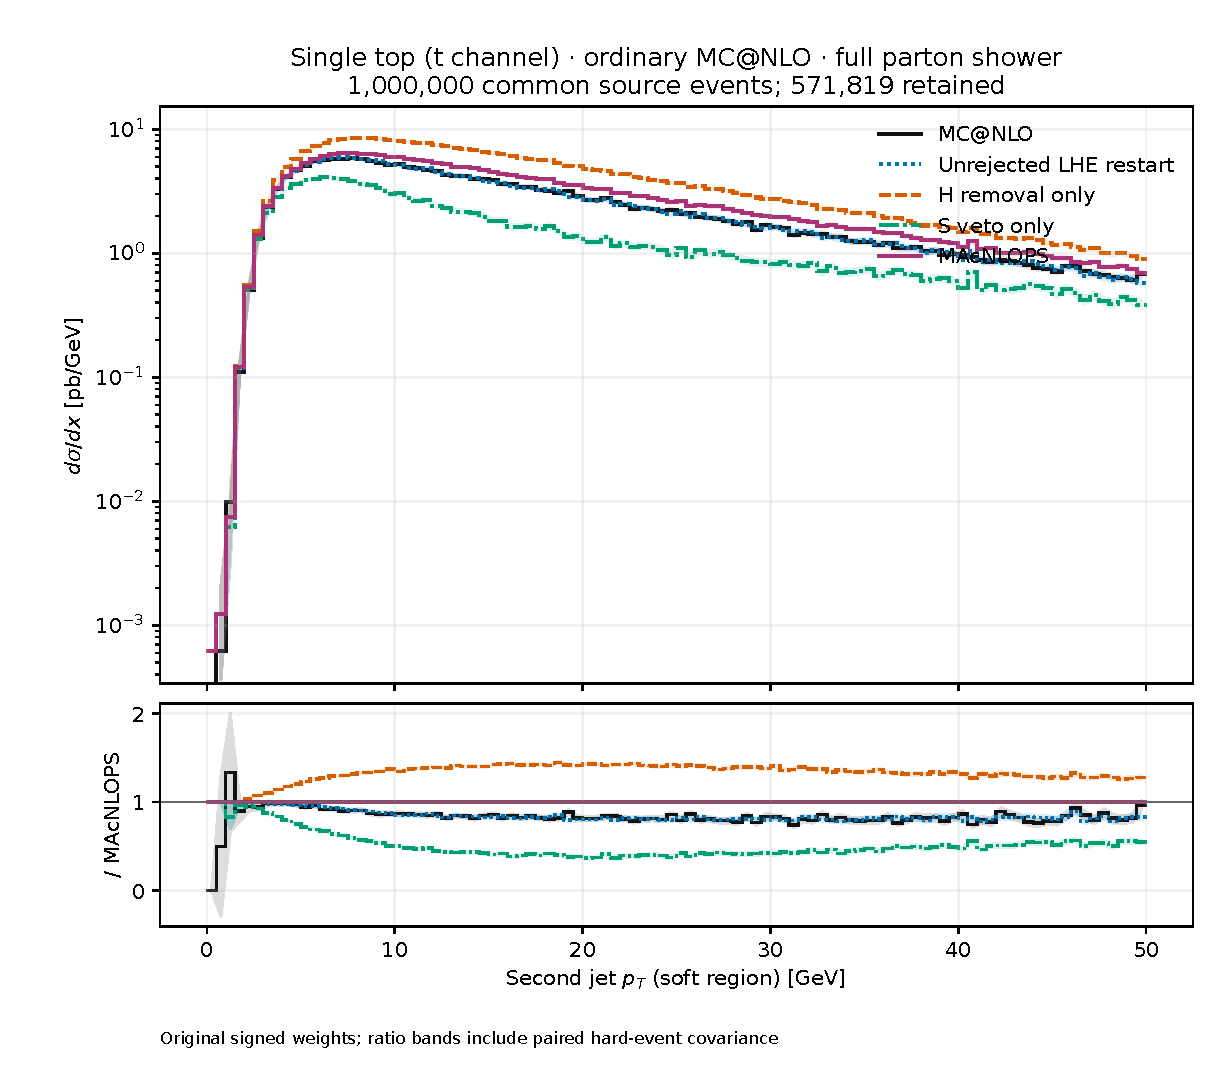
\includegraphics[width=.96\textwidth,height=.72\textheight,keepaspectratio]{figures/full/single_top_ordinary/jet_pt_soft.pdf}
\caption{Global-sum campaign. Single top (5FS), ordinary MC@NLO, full parton shower. The second inclusive jet is shown; the leading jet is the spectator proxy. The soft range is $0$--$50\GeV$ with uniform $0.5\GeV$ bins. The black curve is the uninterrupted reference; blue is the unrejected staged restart. Orange and green isolate H removal and S veto. All ratios use the corresponding combined MAcNLOPS distribution as denominator. Original signed cross-section weights are preserved.}
\label{fig:single_top-ordinary-full}
\end{figure}

\begin{figure}[p]
\centering
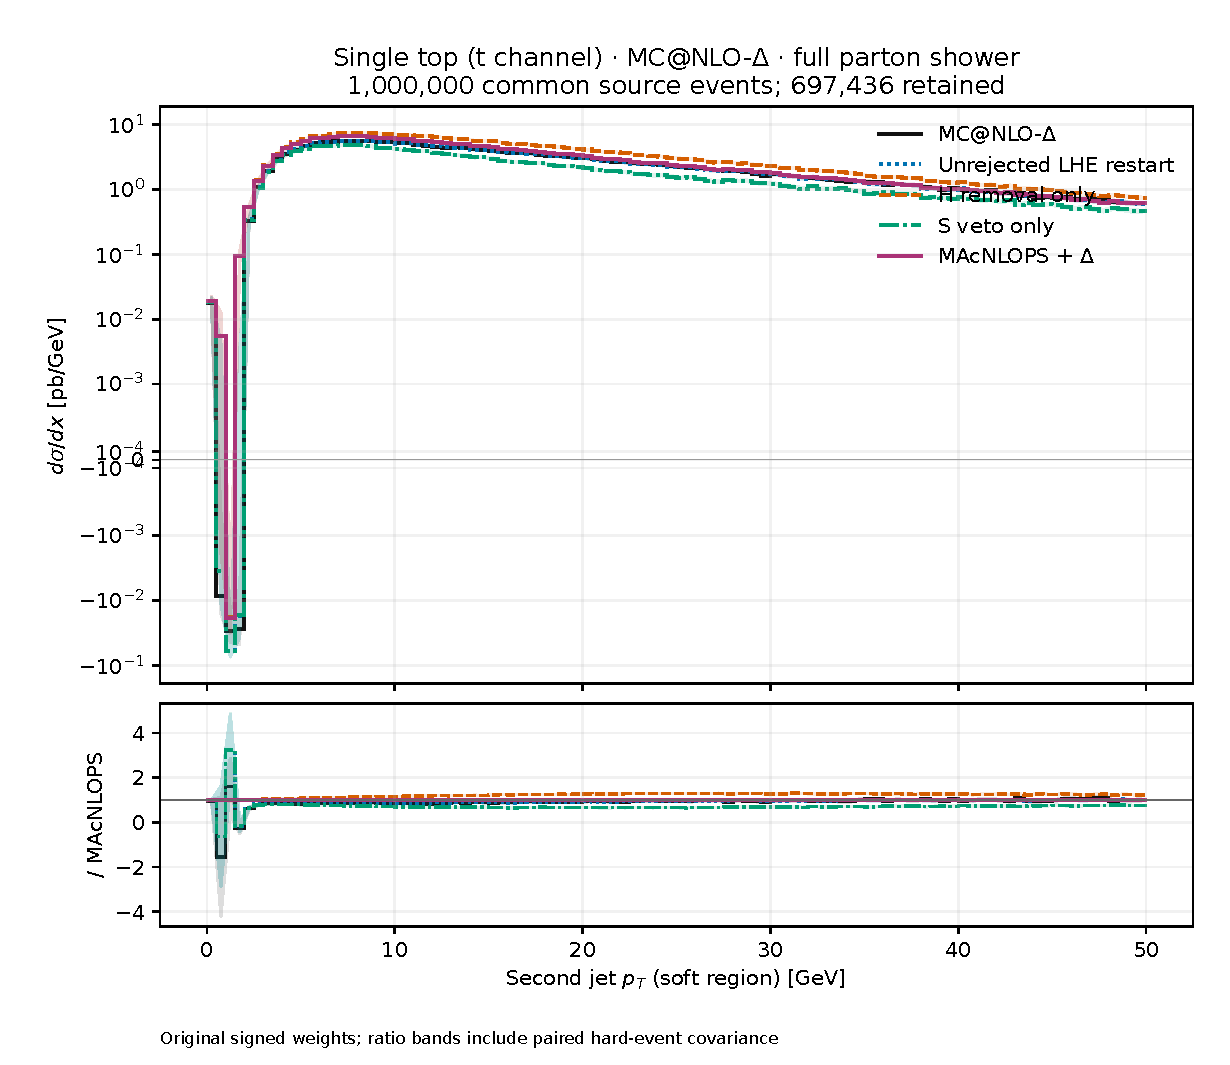
\includegraphics[width=.96\textwidth,height=.72\textheight,keepaspectratio]{figures/full/single_top_delta/jet_pt_soft.pdf}
\caption{Global-sum campaign. Single top (5FS), MC@NLO-$\Delta$, full parton shower. The second inclusive jet is shown; the leading jet is the spectator proxy. The soft range is $0$--$50\GeV$ with uniform $0.5\GeV$ bins. The black curve is the uninterrupted reference; blue is the unrejected staged restart. Orange and green isolate H removal and S veto. All ratios use the corresponding combined MAcNLOPS distribution as denominator. Original signed cross-section weights are preserved.}
\label{fig:single_top-delta-full}
\end{figure}

\begin{figure}[p]
\centering
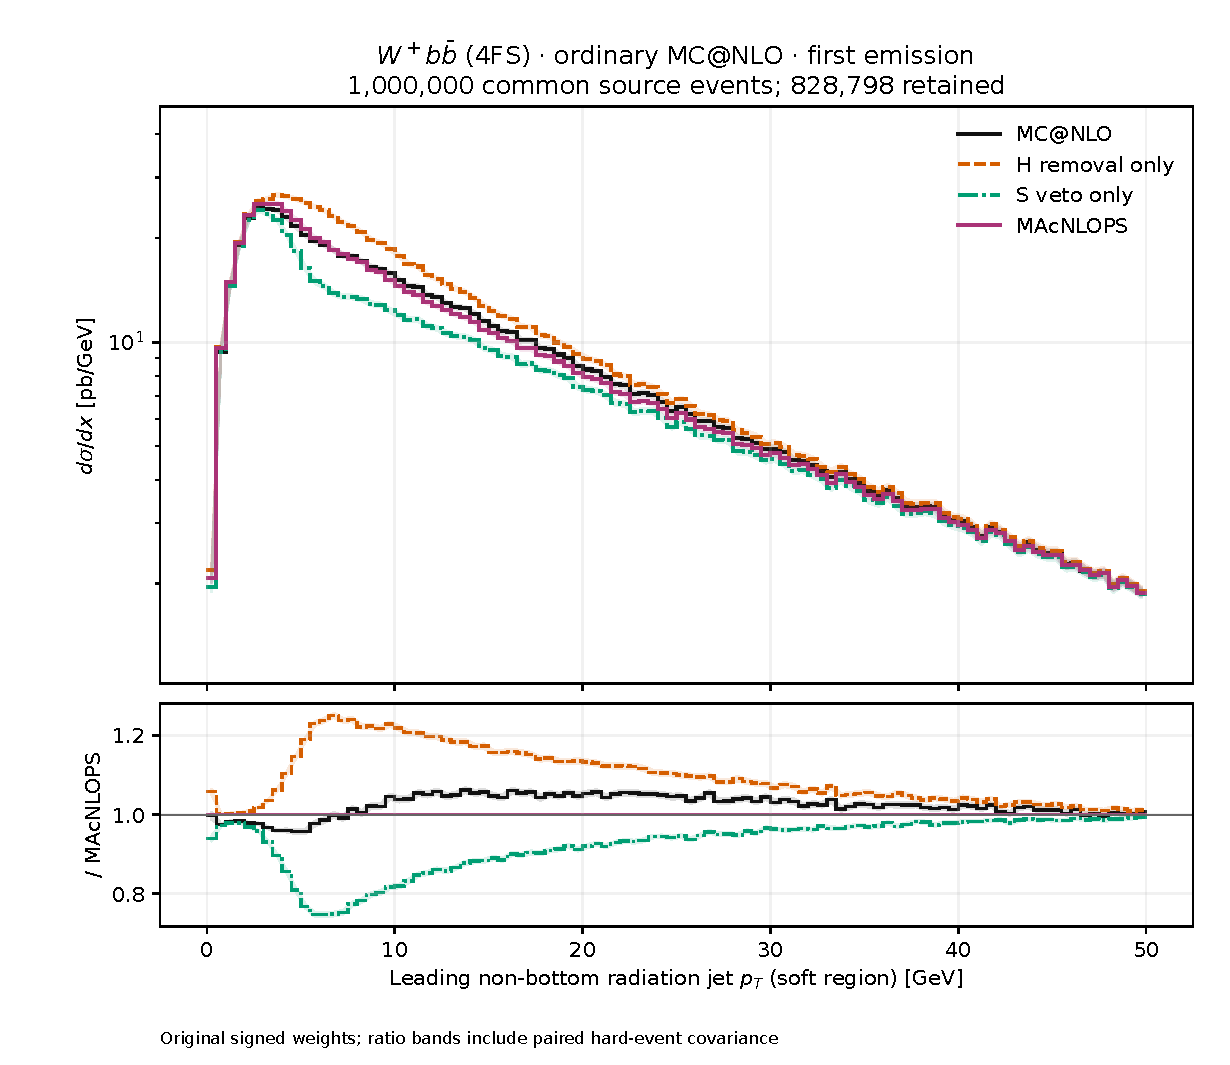
\includegraphics[width=.96\textwidth,height=.72\textheight,keepaspectratio]{figures/first/wbb_ordinary/jet_pt_soft.pdf}
\caption{Global-sum campaign. Wbb (4FS), ordinary MC@NLO, first-emission proposal endpoint. The radiation jets exclude stable bottom partons before clustering. The soft range is $0$--$50\GeV$ with uniform $0.5\GeV$ bins. The black curve is the complete unrejected first-step proposal control, not a separately initialized default-import shower. Orange and green isolate H removal and S veto. All ratios use the corresponding combined MAcNLOPS distribution as denominator. Original signed cross-section weights are preserved.}
\label{fig:wbb-ordinary-first}
\end{figure}

\begin{figure}[p]
\centering
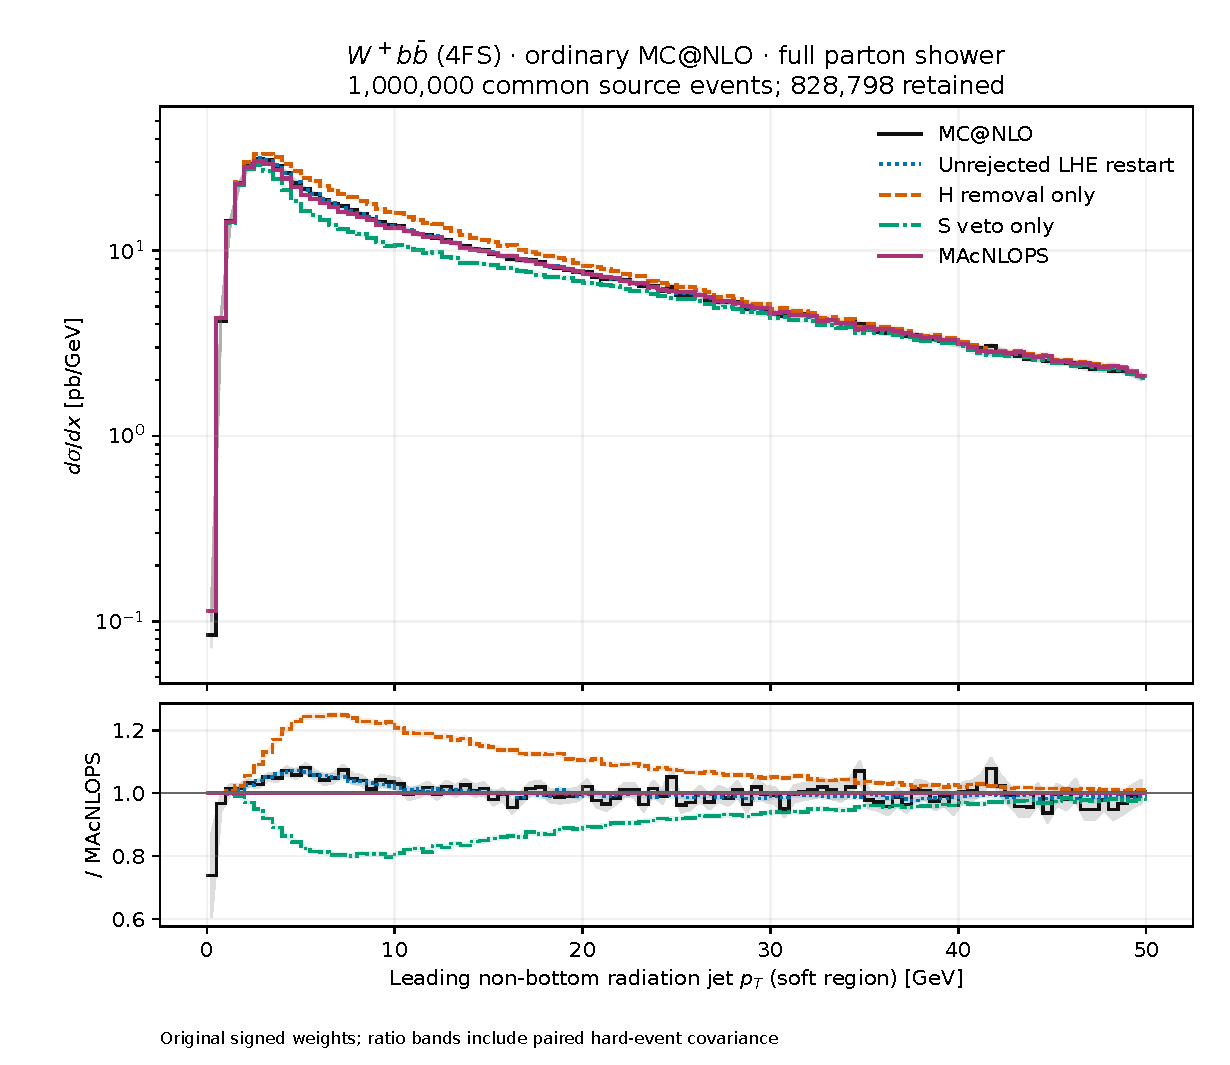
\includegraphics[width=.96\textwidth,height=.72\textheight,keepaspectratio]{figures/full/wbb_ordinary/jet_pt_soft.pdf}
\caption{Wbb (4FS), ordinary MC@NLO, full parton shower. The radiation jets exclude stable bottom partons before clustering. The soft range is $0$--$50\GeV$ with uniform $0.5\GeV$ bins. The black curve is the uninterrupted reference; blue is the unrejected staged restart. Orange and green isolate H removal and S veto. All ratios use the corresponding combined MAcNLOPS distribution as denominator. Original signed cross-section weights are preserved.}
\label{fig:wbb-ordinary-full}
\end{figure}

\begin{figure}[p]
\centering
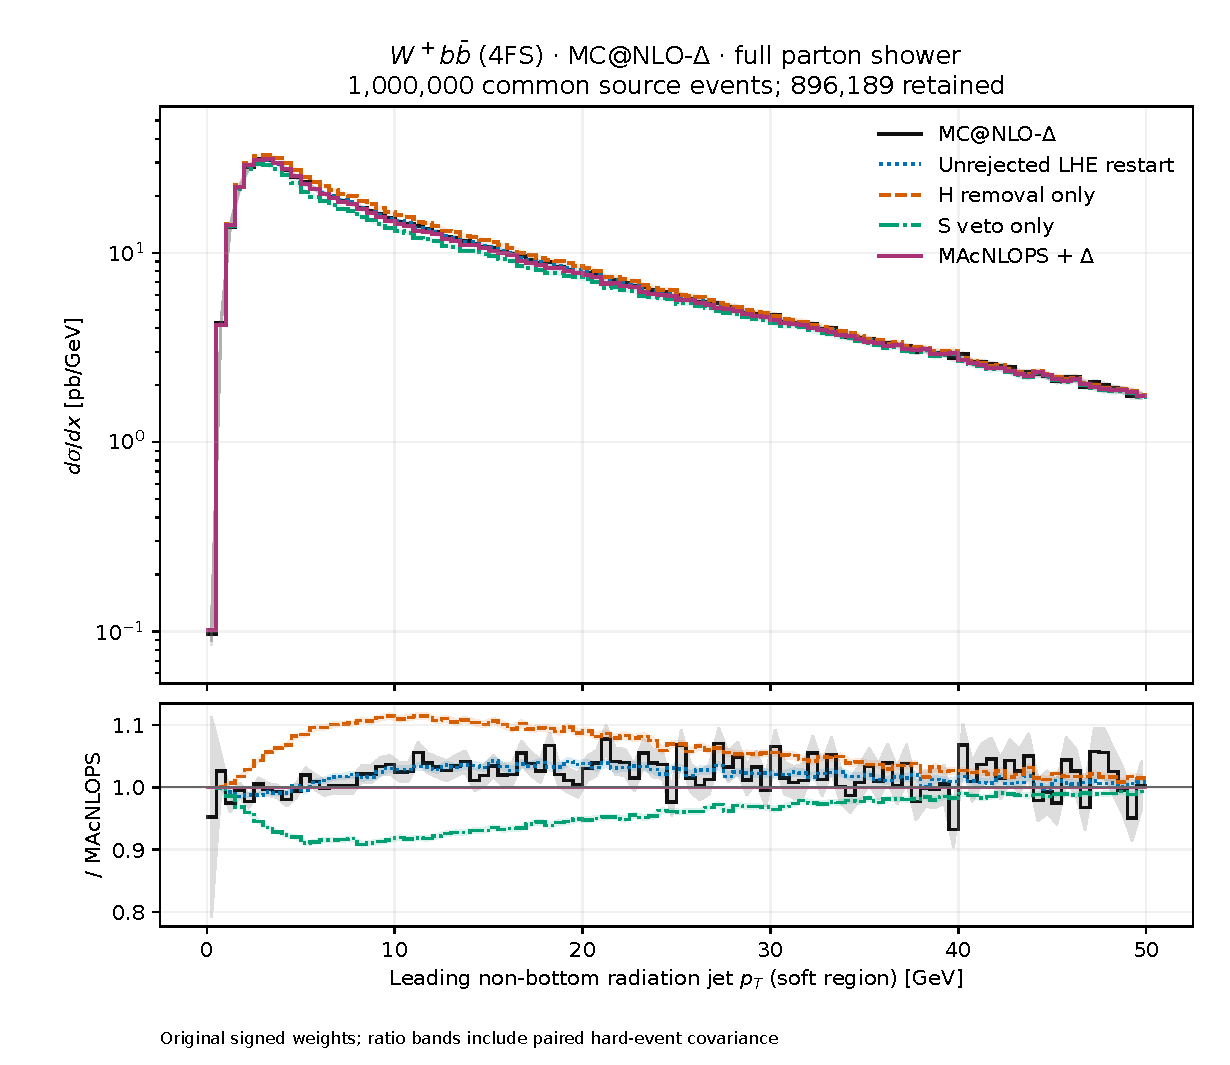
\includegraphics[width=.96\textwidth,height=.72\textheight,keepaspectratio]{figures/full/wbb_delta/jet_pt_soft.pdf}
\caption{Global-sum campaign. Wbb (4FS), MC@NLO-$\Delta$, full parton shower. The radiation jets exclude stable bottom partons before clustering. The soft range is $0$--$50\GeV$ with uniform $0.5\GeV$ bins. The black curve is the uninterrupted reference; blue is the unrejected staged restart. Orange and green isolate H removal and S veto. All ratios use the corresponding combined MAcNLOPS distribution as denominator. Original signed cross-section weights are preserved.}
\label{fig:wbb-delta-full}
\end{figure}

\FloatBarrier
